\documentclass[a4paper, 12pt]{article}
\usepackage[T1]{fontenc}
\usepackage{lmodern}
\usepackage{color}
\usepackage{amsfonts}
\usepackage{epstopdf}
\usepackage{matlab}
%\documentclass{book}
\usepackage{blindtext}
\usepackage{hyperref}
\usepackage[brazil]{babel}
\usepackage{amssymb}
\usepackage[utf8]{inputenc}
\usepackage{amsmath}
\usepackage{indentfirst}
\usepackage{graphicx}
\usepackage{multicol,lipsum}
\usepackage[a4paper,
top=3cm, left=3cm, bottom=3cm, right=3cm]{geometry}
\usepackage{setspace}
\usepackage{multirow}
\usepackage{float}
\usepackage[dvipsnames]{xcolor}
\usepackage[table]{xcolor}
%\usepackage{pdflscape}
\usepackage[DIV=15]{typearea}
\usepackage[nottoc]{tocbibind}
\usepackage[sort,numbers]{natbib}
%\usepackage{cite}
\usepackage{matlab}

\usepackage[utf8]{inputenc}
\usepackage[T1]{fontenc}
\usepackage{lmodern}
\usepackage{graphicx}
\usepackage{color}
\usepackage{hyperref}
\usepackage{amsmath}
\usepackage{amsfonts}
\usepackage{epstopdf}
\usepackage[table]{xcolor}
\usepackage{matlab}


\documentclass[letterpaper]{article}
% bib pack %%%%%%%%%%%%%%%%%%%%%%%%%%%%%%%%%%%%%%%%%%%%%%%%%%%%%%%%%%%%%%%%%%%%%
\usepackage[utf8]{inputenc}
\usepackage{geometry}
    \geometry{left=3cm,right=2cm,top=2cm,bottom=2cm}
%
\usepackage[spanish]{babel}
%
\usepackage[fixlanguage]{babelbib}
    \bibliographystyle{babunsrt}
%
\usepackage{url}

\begin{document}
%\maketitle

\begin{titlepage}
	\begin{center}
		

\vspace{10pt}
%\begin{figure}[H][!ht]
%\centering
%
\includegraphics{puc-rio-logo.png}

%\end{figure}
\begin{figure}[!ht]
\centering

\includegraphics{images/puc-rio-logo.png}
\end{figure}
\huge{Fundamentos de Mecatrônica}
        \vspace{70pt}
        
		\textbf{ENG1731}
		\textbf{\large{\\ }}
		
		\vspace{30pt}
		\textbf{\small{\\Lista 01}}
		\vspace{75pt}
		
	\end{center}
	
	\begin{flushleft}
		\begin{tabbing}
		Aluno(a)\qquad\qquad\=\>Paloma Fernanda Loureiro Sette - 1621595\\
			
			Professor(a)\>João Carlos Virgolino Soares\\
	\end{tabbing}
		  
	\end{flushleft}
	\begin{center}
		%\vspace{\fill}
		\vspace{215pt}
		Rio de Janeiro, 22 de Março de 2023
	\end{center}
\end{titlepage}
%%%%%%%%%%%%%%%%%%%%%%%%%%%%%%%%%%%%%%%%%%%%%%%%%%%%%%%%%%%
\newpage
\tableofcontents
\thispagestyle{empty}

\newpage
\pagenumbering{arabic}

\newpage

%\newcommand{\listequationsname}{Lista de Equações}
%\newlistof{myequations}{equ}{\listequationsname}
%\newcommand{\myequations}[1]{%
%\addcontentsline{equ}{myequations}{\protect\numberline{\theequation}#1}\par}

%\listofmyequations
\newpage


\newpage

\listoffigures
\thispagestyle{empty}

\newpage
%%%%%%%%%%%%%%%%%%%%%%%%%%%%%%%%%%%%%%%%%%%%%%%%%%%%%%%%%
%%%%%%%%%%%%%%%%%%%%%%%%%%%%%%%%%%%%%%%%%%%%%%%%%%%

\newpage

\thispagestyle{empty}

\newpage

\section{Introdução}
Este relatório refere-se ao primeiro trabalho da disciplina de Fundamentos de Mecatrônica, ENG1731, de 2023.1. 

Trataremos de modelagem e simulação de um sistemaa mecânico massa-mola-amortecedor, utilizando Simulink e MATLAB.

\section{Questão 01}
Para a resolução dos seguintes itens que se encontram separados por subtópicos, consideremos a figura a seguir, que mostra um sistema massa-mola-amortecedor com massa \textbf{m} atrelada a uma mola de constante \textbf{$k$} e a um amortecedor de constante \textbf{$b$}.

\begin{figure}[H]
\centering

\includegraphics[scale = 0.8]{images/sistema.png}
\label{filtro1}
\caption{Sistema massa-mola-amortecedor - questão 01}
\end{figure}

\subsection{Modelo matemático do sistema}

Sabemos que:

\begin{equation}
    F_{b} = b\dot x
\end{equation}

\begin{equation}
    F_{k} = k x
\end{equation}

O somatório de forças vetoriais será: 

\begin{equation}
    \sum{\vec{F}} = \vec{F_{k}} + \vec{F_{b}} + \vec{F} = m\ddot x
\end{equation}

No entanto, como a força $F$ está agindo no sentido negativo (para a esquerda), teremos,

\begin{equation}
    m\ddot x = F - b\dot x - kx 
\end{equation}

Logo, o modelo matemático do sistema pode ser representado pela equação \ref{model_mat}:

\begin{equation}\label{model_mat}
    \ddot x = \frac{1}{m} (F-b \dot x - kx )
\end{equation}

\subsection{Resposta Dinâmica}
Com base no modelo matemático obtido no tópico anterior, encontramos a resposta dinâmica do sistema (posição bloco em função do tempo) utilizando o Simulink.

\begin{figure}[H]
\centering
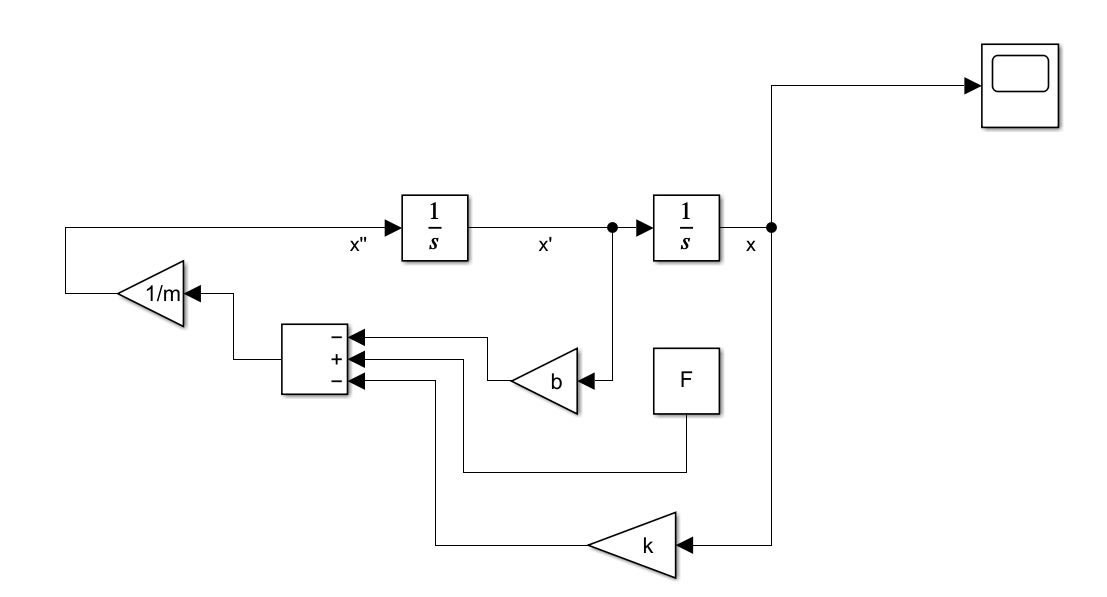
\includegraphics[scale = 0.7]{images/simulink_resposta_dinamica.png}
\label{filtro1}
\caption{Sistema modelado com o Simulink}
\end{figure}

\subsection{Definição dos Parâmetros}
% This LaTeX was auto-generated from MATLAB code.
% To make changes, update the MATLAB code and export to LaTeX again.

No MATLAB, criamos um script para a definição dos parâmetros do sistema que foi compilado no Simulink.

\sloppy
\epstopdfsetup{outdir=./}
\graphicspath{ {./L01_Latex_images/} }


\begin{matlabcode}
%% LISTA 01
close all
clear
clc

%definição dos parâmetros

% Sistema massa-mola-amortecedor

x0      = 0.5;        % m
k       = 50;         % N/m
b       = 10;         % Ns/m
m       = 5;          % kg
F       = 20;         % N

\end{matlabcode}



\subsection{Resposta Gráfica}
Com o auxílio do script criado, geramos os gráficos de posição em função do tempo, usando os parâmetros iniciais.

\begin{figure}[H]
\centering
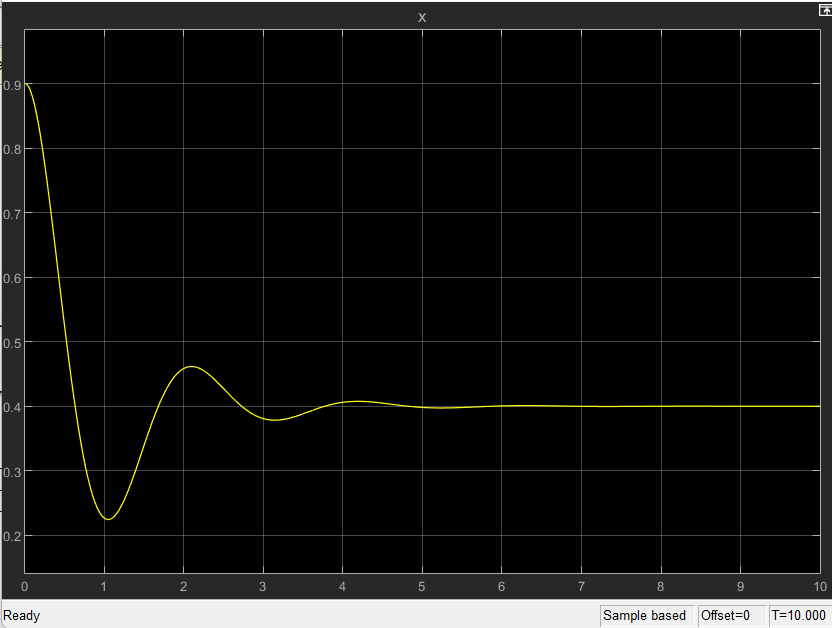
\includegraphics[scale = 0.8]{images/graph_simulink.png}
\label{filtro1}
\caption{Resposta gráfica gerada com o Simulink}
\end{figure}



\subsection{Solução analítica (homogênea)}
A partir do modelo matematico, podemos encontrar a solução analítica. Tirando as raízes do polinômio característico, verificamos que as mesmas são complexas. 

Então, primeiramente, sabemos que nossa equação homogênea será na forma:

\begin{equation}
    {\mathrm{e}}^{\alpha t} \,{\left(C_1 \,\cos \left(\beta\,t\right) + C_2 \,\sin \left(\alpha\,t\right)\right)}
\end{equation}

onde 

\begin{equation*}
    \lambda_{1,2} = \alpha \pm \beta j
\end{equation*}

\sloppy
\epstopdfsetup{outdir=./}
\graphicspath{ {./untitled4_images/} }

\begin{document}

\begin{matlabcode}
%% LISTA 01
clear; clc;

x0      = 0.5;        % m
k       = 50;         % N/m
b       = 10;         % Ns/m
m       = 5;          % kg
F       = 20;         % N

delta = b^2 - (4*m*k);
lambda = (-b -sqrt(delta))/(2*m)
\end{matlabcode}
    
\begin{matlaboutput}
lambda = -1.0000 - 3.0000i
\end{matlaboutput}
\begin{matlabcode}

alpha = -1
\end{matlabcode}
\begin{matlaboutput}
alpha = -1
\end{matlaboutput}
\begin{matlabcode}
beta = -3
\end{matlabcode}
\begin{matlaboutput}
beta = -3
\end{matlaboutput}

Logo, podemos desenvolver nosssa equação homogênea. Como temos que nossa posição inicial é $0.5m$, podemos descobrir o valor de $C_1$ com $x(0) = 0.5$.

\begin{equation*}
    x(0) = \frac{1}{2} = {\mathrm{e}}^{0} * (C_1cos(0) + C_2 sin(0))
\end{equation*}

Logo,

\begin{equation*}
    x(0) = \frac{1}{2} = C_1
\end{equation*}

Agora que sabemos o valor de $C_1$, podemos chegar em $C_2$.

Derivando $x(t)$, teremos:

\begin{equation*}
    \dot x (t) = - {\mathrm{e}}^{-t} * (C_1 cos(3t) - C_2 sin(3t)) - {\mathrm{e}}^{-t} * (3 C_2 cos(3t) + 3C_1 sin(3t))
\end{equation*}

Então, fazendo $\dot x(0) = 0$, podemos descobrir o valor de $C_2$:

\begin{equation*}
    \dot x (0) = 0 = - {\mathrm{e}}^{0} * (C_1 cos(0) - C_2 sin(0)) - {\mathrm{e}}^{0} * (3 C_2 cos(0) + 3C_1 sin(0))
\end{equation*}

\begin{equation*}
    0 = - 1 * (\frac{1}{2} * 1) - 1 * (3 C_2 *1)
\end{equation*}

\begin{equation*}
    C_2 = - \frac{1}{6}
\end{equation*}

E podemos notar que

\begin{equation*}
    C_2 = - \frac{C_1}{\beta}
\end{equation*}


\begin{matlabcode}

No MATLAB, colocamos:

t   = 0:0.001:10;
C1  = x0;
C2  = -C1/beta;

% Equação homogênea
xh = exp(alpha.*t).*(C1.*cos(beta.*t) + C2.*sin(alpha.*t));
\end{matlabcode}








\subsection{Solução analítica (particular)}
Para a solução particular, partimos do princípio dos coeficientes a determinar. 
Como temos um caso de força constante, temos que, no caso de um deslocamento na condição de equilíbrio, nossa solução particular será:
\begin{equation}
    x_p = \frac{F}{k}
\end{equation}
Então, declaramos no MATLAB para encontrar o valor numérico:
\begin{matlabcode}

% Solução particular xp(t), para uma força constante.
xp = F/k
\end{matlabcode}

\begin{matlaboutput}
xp = 0.4000
\end{matlaboutput}


\subsection{Resposta gráfica (sol. analítica)}

\begin{matlabcode}
    
    plot(t, Xh+xp);
    grid on
    
\end{matlabcode}


\begin{figure}[H]
\centering
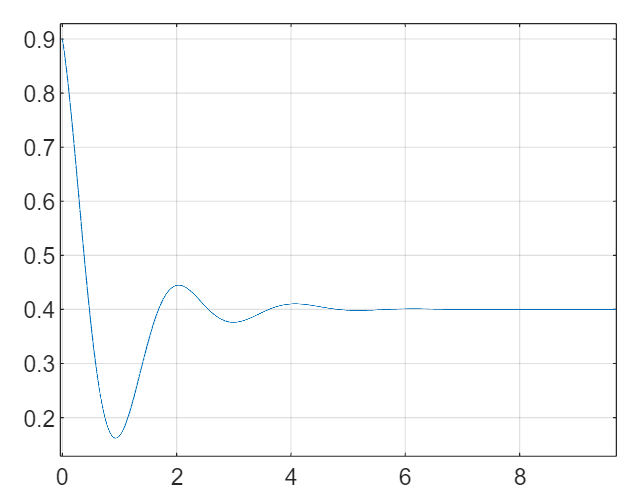
\includegraphics[scale = 0.8]{images/graph_script.PNG}
\label{filtro1}
\caption{Gráfico da solução analítica gerado}
\end{figure}

\subsubsection{Comparação com o Simulink}

Como podemos observar, ao compararmos as respostas do gráfico do Simulink com o do script, obtivemos as respostas parecidas, o que satisfaz as nossas simulações.

\begin{figure}[H]
\centering
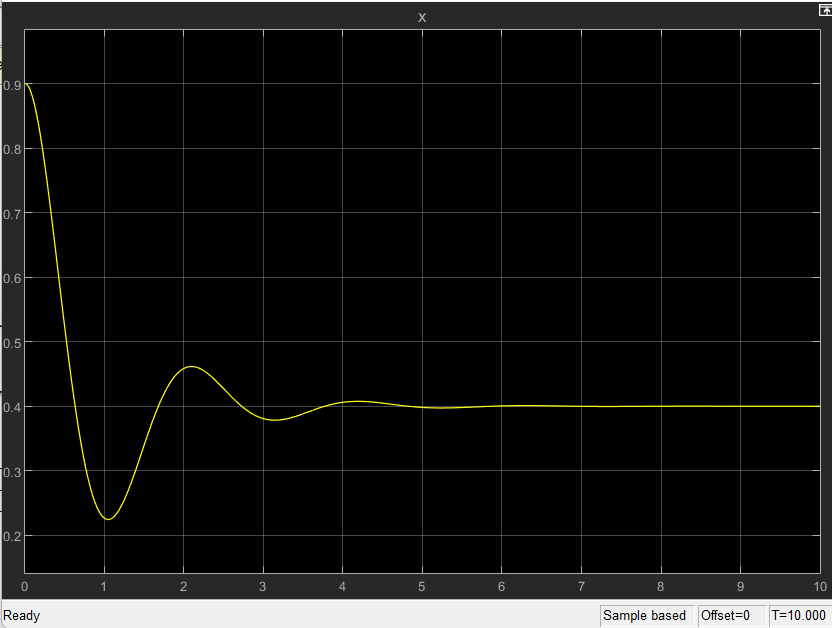
\includegraphics[scale = 0.50]{images/graph_simulink.png}
\label{filtro1}
\caption{Gráfico do Simulink}
\end{figure}

\begin{figure}[H]
\centering
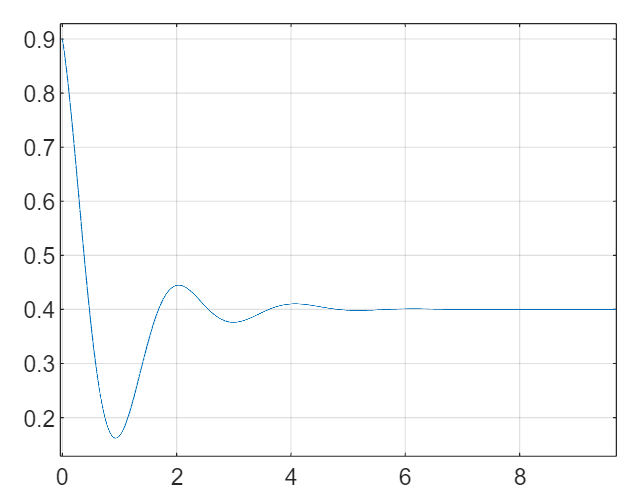
\includegraphics[scale = 0.50]{images/graph_script.PNG}
\label{filtro1}
\caption{Gráfico gerado no Script analiticamente}
\end{figure}


\newpage
% REFERENCIAS %%%%%%%%%%%%%%%%%%%%%%%%%%%%%%%%%%%%%%%%%%%%%%%%%%%%%%%%%%%%%%
    \nocite{*}
    \bibliography{src/bibliography}
    
\end{document}
\section{Referências Bibliográficas}



\end{document}